\documentclass{beamer}

\useoutertheme[height=0.1\paperheight,width=0.1\paperwidth,hideothersubsections]{sidebar}
\usecolortheme{whale}
\usecolortheme{orchid}

\useinnertheme[shadow]{rounded}
\setbeamercolor{title page}{fg=blue!70,bg=blue}
\setbeamercolor{logo}{bg=blue!60}
\setbeamercolor{frametitle}{fg=black,bg=blue!60}
%\setbeamercolor{section in sidebar}{fg=red}
\setbeamercolor{block title}{bg=blue!28!white,fg=blue}
\setbeamercolor{block body}{bg=red!15!white}
\setbeamercolor{sidebar}{bg=blue!70}

\setbeamertemplate{background canvas}[vertical shading][bottom=white,top=blue!25]
\usefonttheme{serif}
\setbeamertemplate{navigation symbols}{}
\usepackage{CJKutf8}
%\usepackage{subfigure}
\usepackage{xmpmulti}
\usepackage{colortbl,dcolumn}
\graphicspath{{October/}}
\DeclareGraphicsRule{*}{mps}{*}{}

\logo{
\includegraphics[width=0.1\paperwidth]{huoqiang.jpg}}
\renewcommand{\raggedright}{\leftskip=0pt \rightskip=0pt plus 0cm}
\raggedright
\def\hilite<#1>{\temporal<#1>{\color{blue!35}}{\color{magenta}}{\color{blue!75}}}

\newcolumntype{H}{>{\columncolor{blue!20}}c!{\vrule}}
\newcolumntype{H}{>{\columncolor{blue!20}}c}
\newcommand{\upcite}[1]{\textsuperscript{\cite{#1}}}
\bibliographystyle{plain}
\newcommand{\yihao}{\fontsize{30pt}{\baselineskip}\selectfont}
\newcommand{\sihao}{\fontsize{14pt}{\baselineskip}\selectfont}
\newcommand{\xiaosihao}{\fontsize{12pt}{\baselineskip}\selectfont}
\newcommand{\wuhao}{\fontsize{10.5pt}{\baselineskip}\selectfont}  
\newcommand{\xiaowuhao}{\fontsize{9pt}{\baselineskip}\selectfont} 
\newcommand{\liuhao}{\fontsize{7.875pt}{\baselineskip}\selectfont}
\newcommand{\qihao}{\fontsize{5.25pt}{\baselineskip}\selectfont}
\newcommand{\ThankYouPage}{
  \begin{frame}
    \yihao \centering \textcolor{blue}
    {Thank You!}
  \end{frame}
}

\begin{document}
\begin{CJK*}{UTF8}{gkai}
  \title{十月工作总结}
  \author[\textcolor{black}{作者 朱海文}]{作者~~\textcolor{olive}{朱海文}}
  \institute{\textcolor{violet}{摩科特医疗器械有限公司}}
  \date{\today}
  \frame{\titlepage}
  %======================================================
  \section*{目录}
  \frame{\frametitle{目录}\tableofcontents}
  \section{一块探测器模块的模拟结果}
  \begin{frame}\frametitle{探测器晶粒几何}
    \begin{minipage}[t]{0.3\textwidth}
      \liuhao
      探测器晶粒共$24\times24$块,如果将中间的两块小晶粒合并成一块,则有
      $24\times16$块,列数为0-17列的
      即为合并之后的结果,事例数为($3.6\times10^8$)。
      
      晶粒编号从左至右为第i列($0\leq i \leq 25$),从上至下为
      第j行($100\le j \le2400$),在保存的时候将行数乘以100,以便区分行和列。
    \end{minipage}
    \begin{minipage}[t]{0.7\textwidth}
      \begin{figure}[ht]
	\centering
        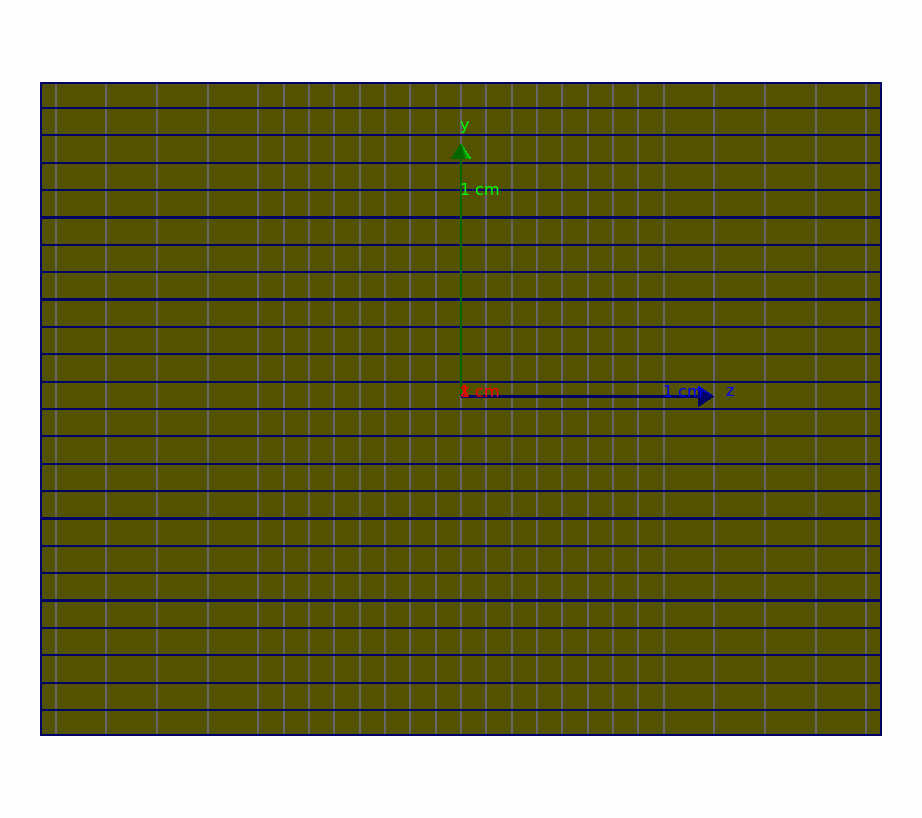
\includegraphics[width=0.9\textwidth,height=0.7\textwidth]{Detector.png}
	\caption{\liuhao 探测器晶粒}
	\label{Detector}
      \end{figure}
    \end{minipage}
  \end{frame}
  %----------------------------
  \subsection{无准直器}
  \begin{frame}\frametitle{无准直器}
    \begin{minipage}[t]{0.3\textwidth}
      \liuhao
      分有准直器和没准直器两种情况模拟,右图分别是无准直器时直射和散射到每块探测器单元的能量,编号为0和
      17的两列是边缘处宽度为$0.5mm$的两列,中间块的宽度为$1.915mm$(或者$0.915mm\times 2$);编号为1和24的两行
      也比中间的行窄,故这些晶体上的能量比中间的晶体上能量要小。
    \end{minipage}
    \begin{minipage}[t]{0.7\textwidth}
      \vskip -0.5cm
      \begin{figure}[ht]
        \centering
        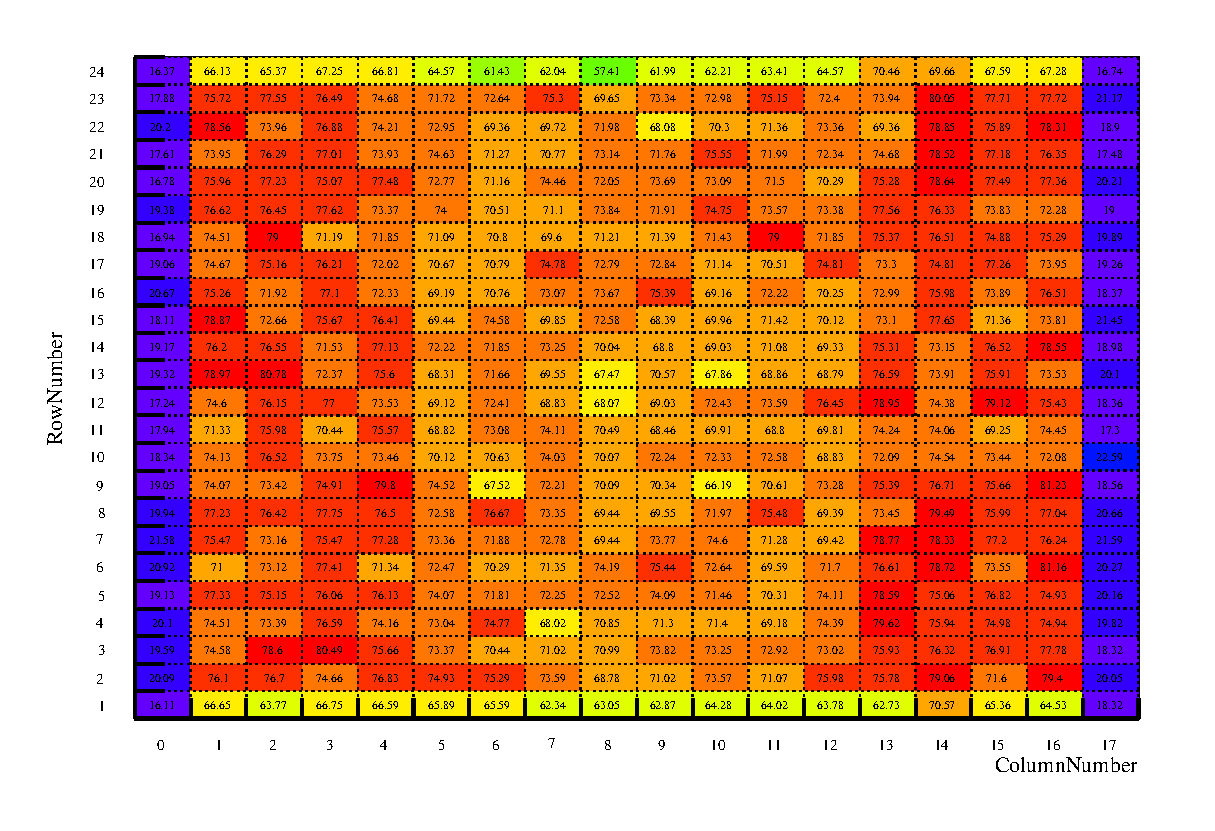
\includegraphics[width=\textwidth,height=0.58\textwidth]{WithoutCollimatorDirectEnergyMerged.eps}

        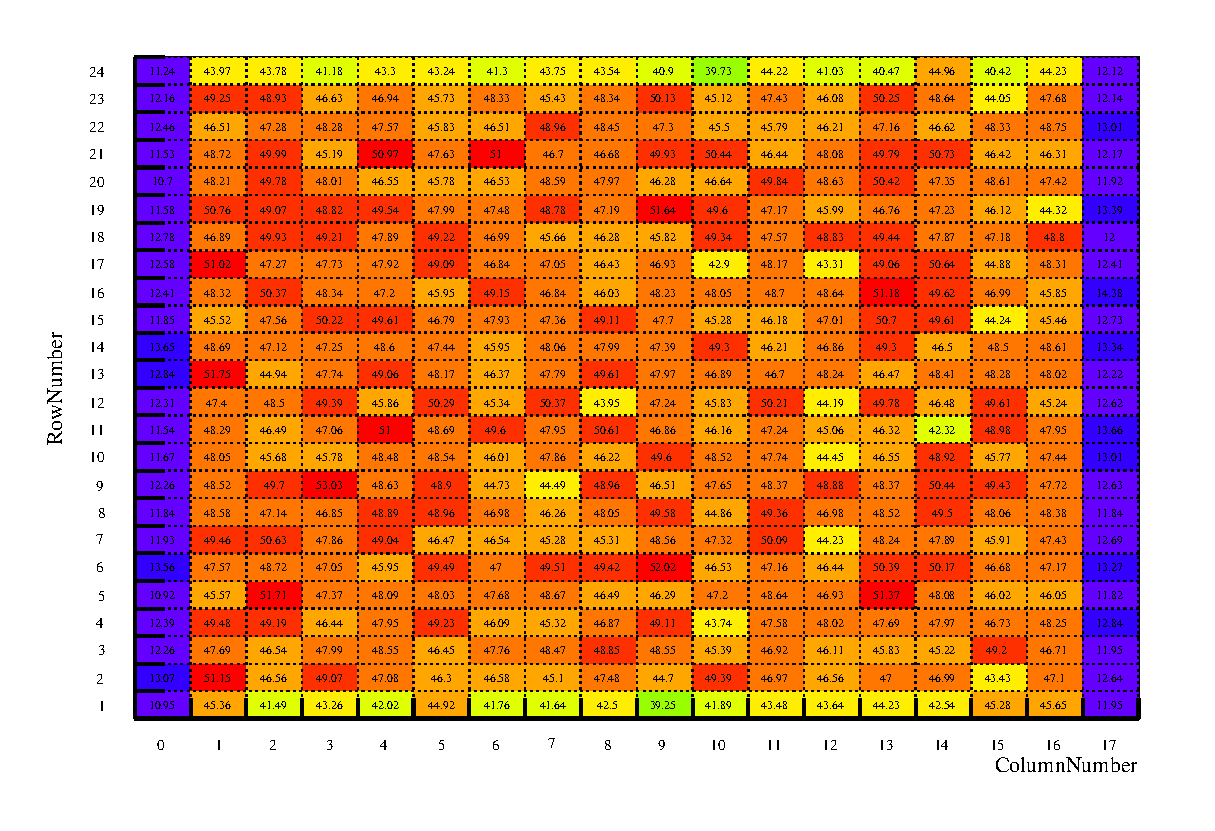
\includegraphics[width=\textwidth,height=0.58\textwidth]{WithoutCollimatorScatteringEnergyMerged.eps}
      \end{figure}
    \end{minipage}
  \end{frame}
  %----------------------------
  \begin{frame}\frametitle{无准直器散射能量所占的比例}
    \begin{figure}[ht]
      \centering
      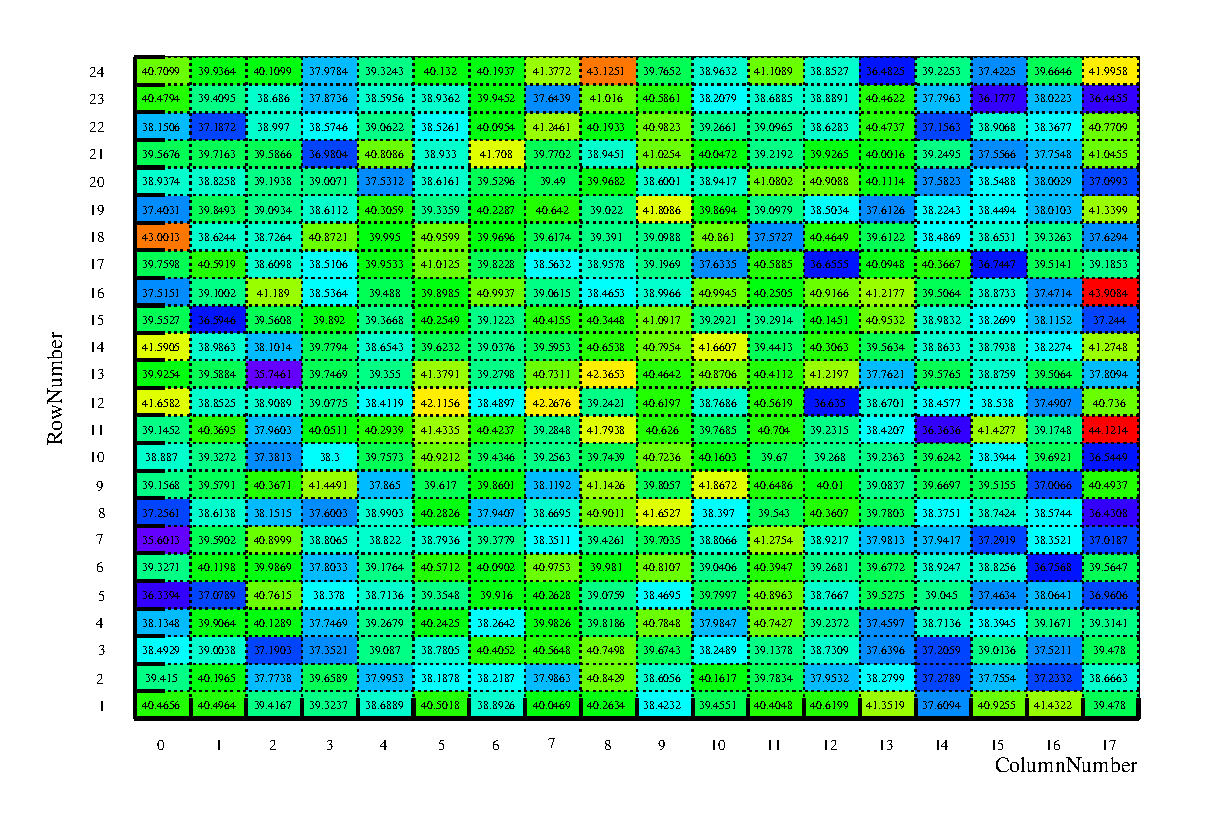
\includegraphics[width=\textwidth]{WithoutCollimatorScatteringRatioMerged.eps}
    \end{figure}
    \liuhao
    \vskip -1cm
    \begin{itemize}
      \item 由于大角散射的存在,实际上24块模块中散射能量占的比例会比这个值大。
    \end{itemize}
  \end{frame}
 %----------------------------
  \subsection{有准直器}
  \begin{frame}\frametitle{有准直器}
    \begin{minipage}[t]{0.7\textwidth}
      \vskip -0.5cm
      \begin{figure}[ht]
        \centering
        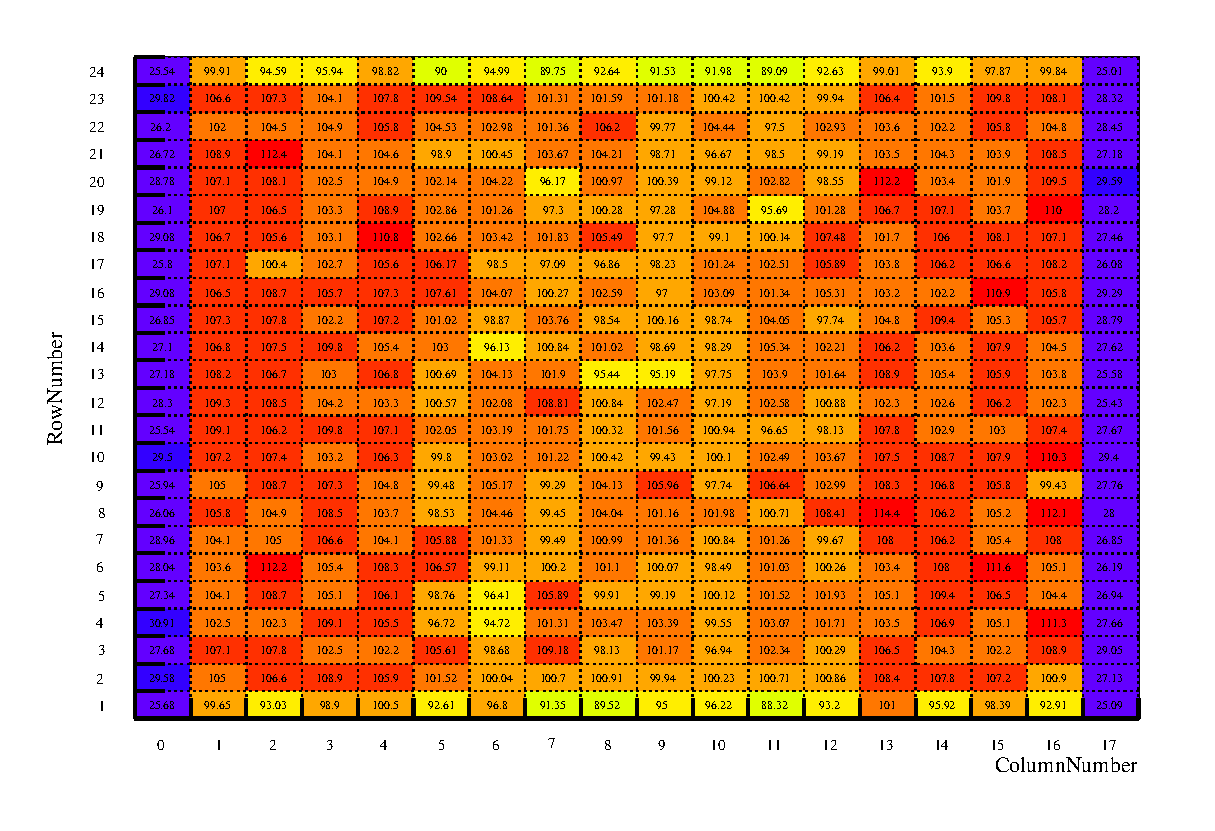
\includegraphics[width=\textwidth,height=0.58\textwidth]{WithCollimatorDirectEnergyMerged.eps}
        
        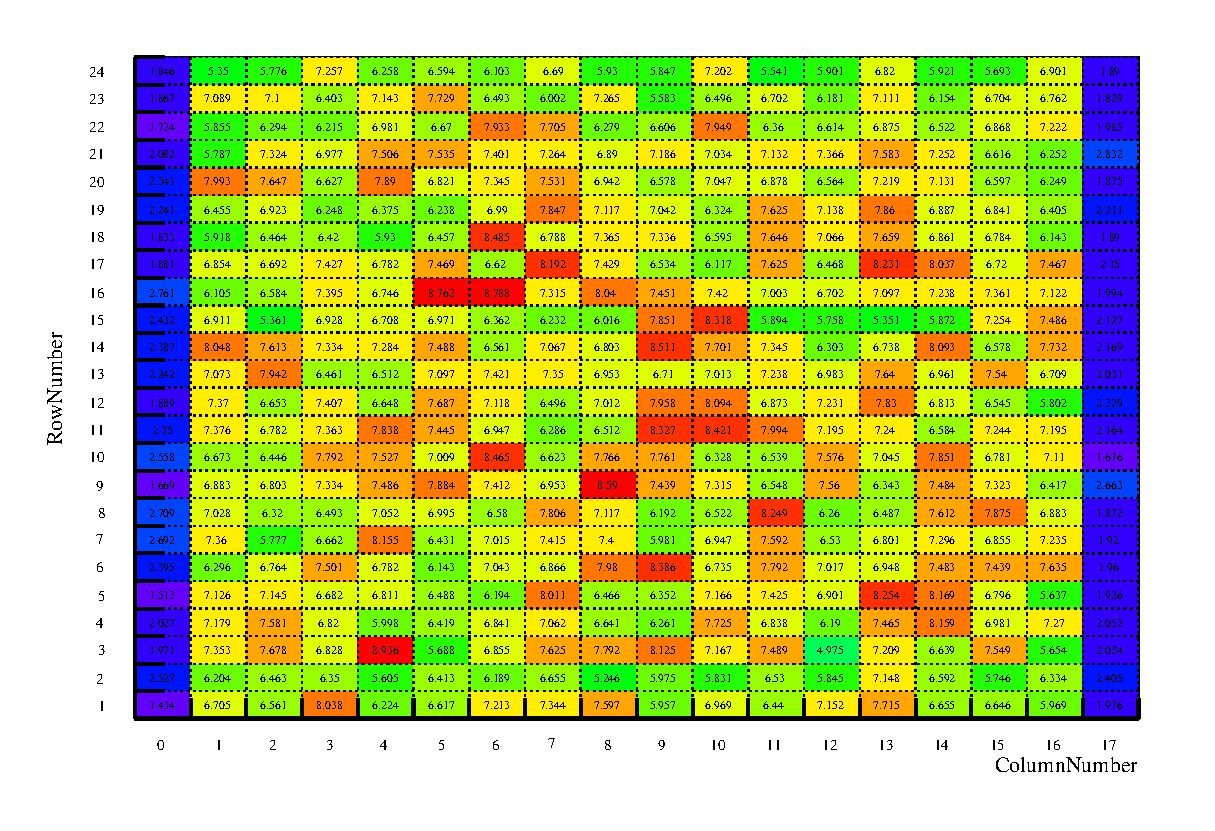
\includegraphics[width=\textwidth,height=0.58\textwidth]{WithCollimatorScatteringEnergyMerged.eps}
      \end{figure}
    \end{minipage}
    \begin{minipage}[t]{0.29\textwidth}
      \vskip 1cm
      \liuhao
      可以看到有准直器时,第1行和第24行散射的能量比中间的多,这是由于只放了一块探测器模块与一块准直器,
      会从准直器外面散射进入部分能量。
      \begin{figure}[ht]
	\centering
	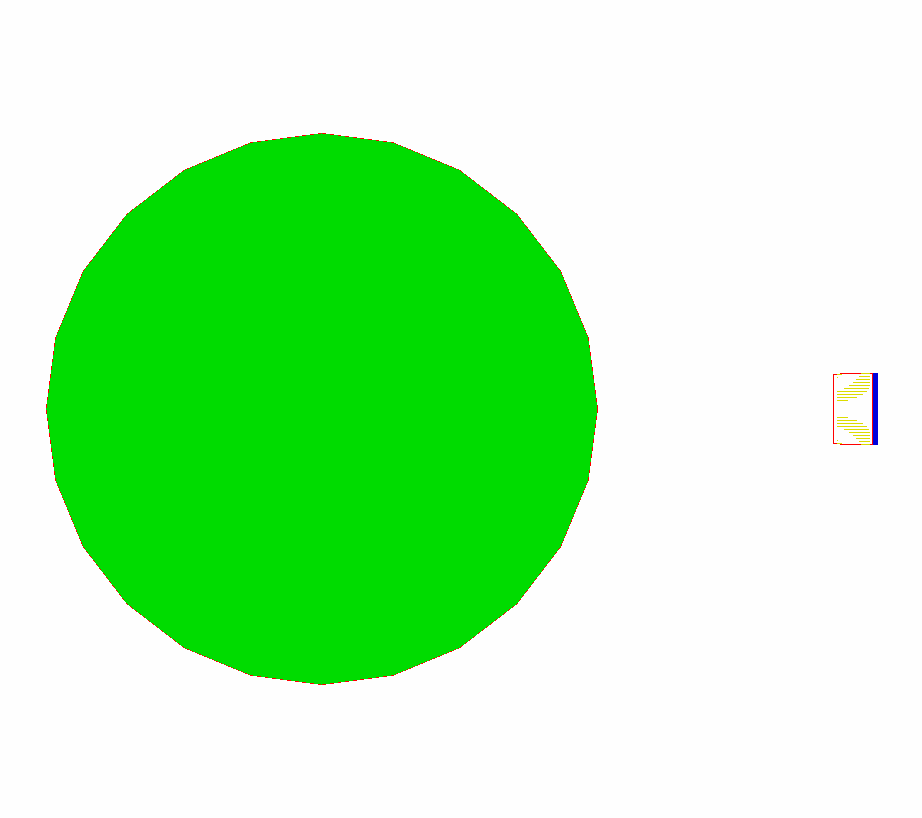
\includegraphics[width=\textwidth]{SingleCollimator.png}
      \end{figure}
    \end{minipage}
  \end{frame}
  %----------------------------
  \begin{frame}\frametitle{有准直器散射能量所占的比例}
    \begin{figure}[ht]
      \centering
      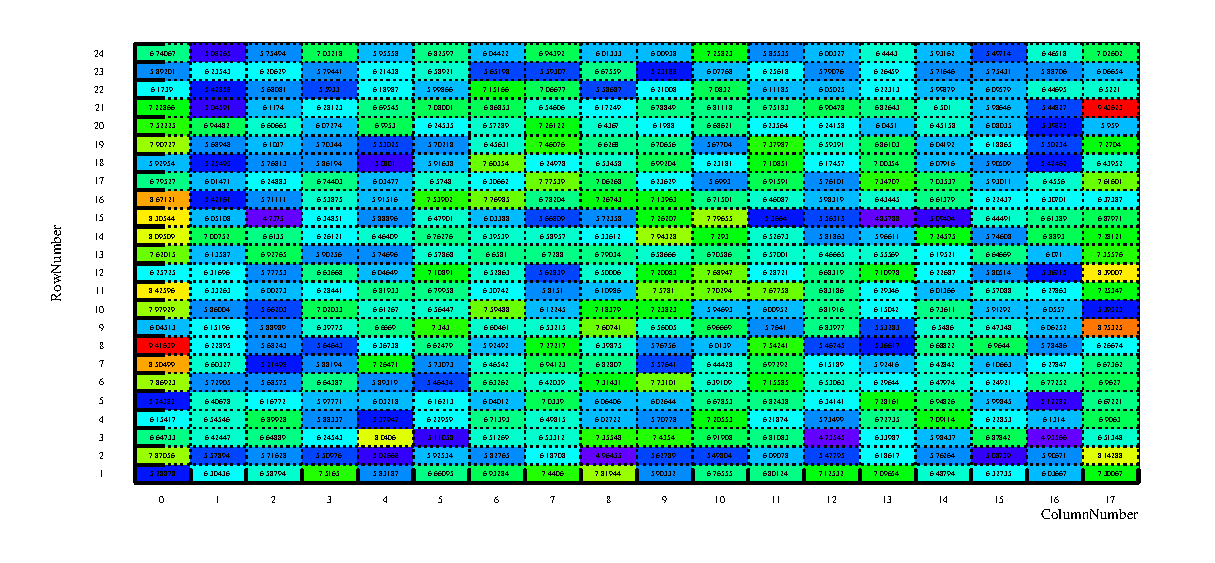
\includegraphics[width=\textwidth]{WithCollimatorScatteringRatioMerged.eps}
      \caption{\liuhao有准直器时散射的比例(\%)}
    \end{figure}
  \end{frame}
  %-----------------------------------
  \section{140keV电子打靶模拟}
  \begin{frame}\frametitle{穿过挡板之后的能普}
    \begin{minipage}[t]{0.29\textwidth}
      \liuhao
      \begin{itemize}
	\item 首先模拟能量为$140keV$的电子轰击钨靶,得到产生的射线的能普;
	\item 按照得到的能普进行抽样,模拟射线穿过不同厚度的铝和铜之后的能普;
	\item 统计不同能量阈值下的光子数所占的比例。
      \end{itemize}
    \end{minipage}
    \begin{minipage}[t]{0.7\textwidth}
      \vskip -0.4cm
      \begin{figure}[ht]
        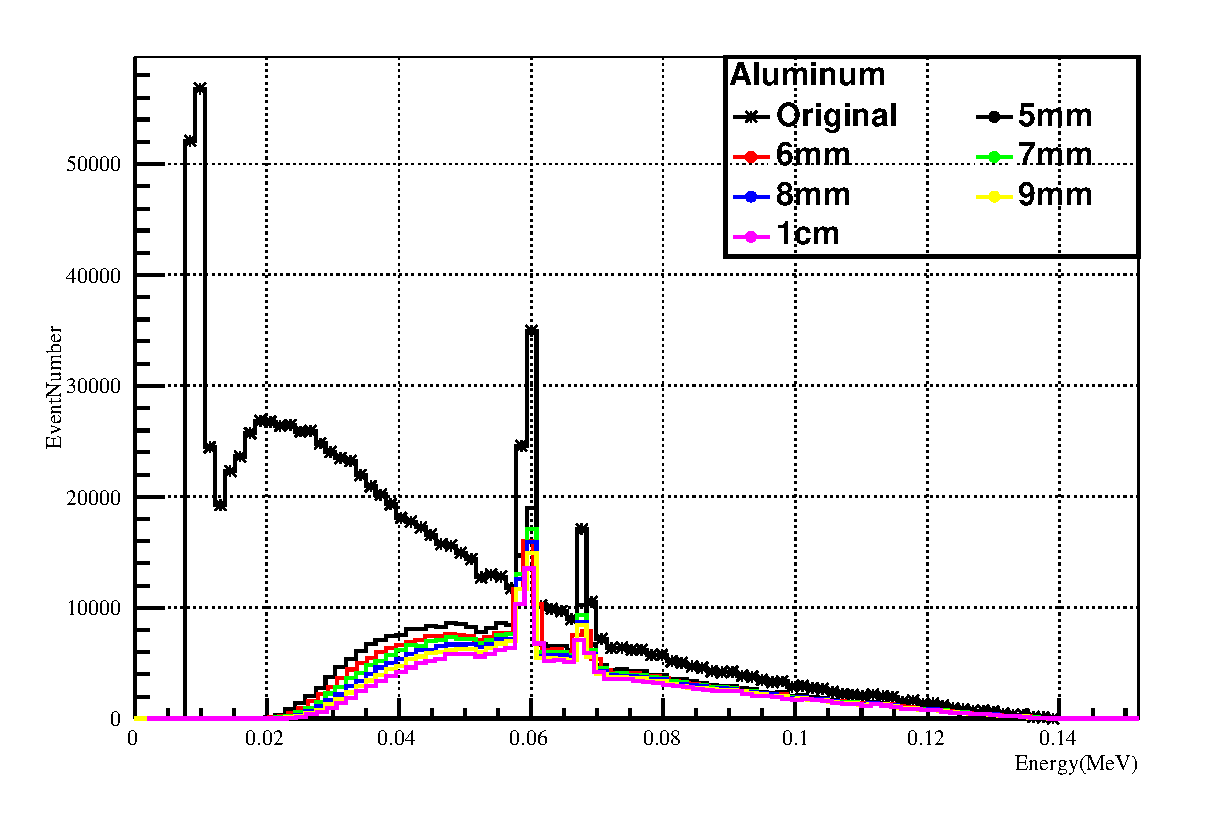
\includegraphics[width=\textwidth,height=0.58\textwidth]{140keVelectronEnergyAfterAluminumApron.eps}
        
	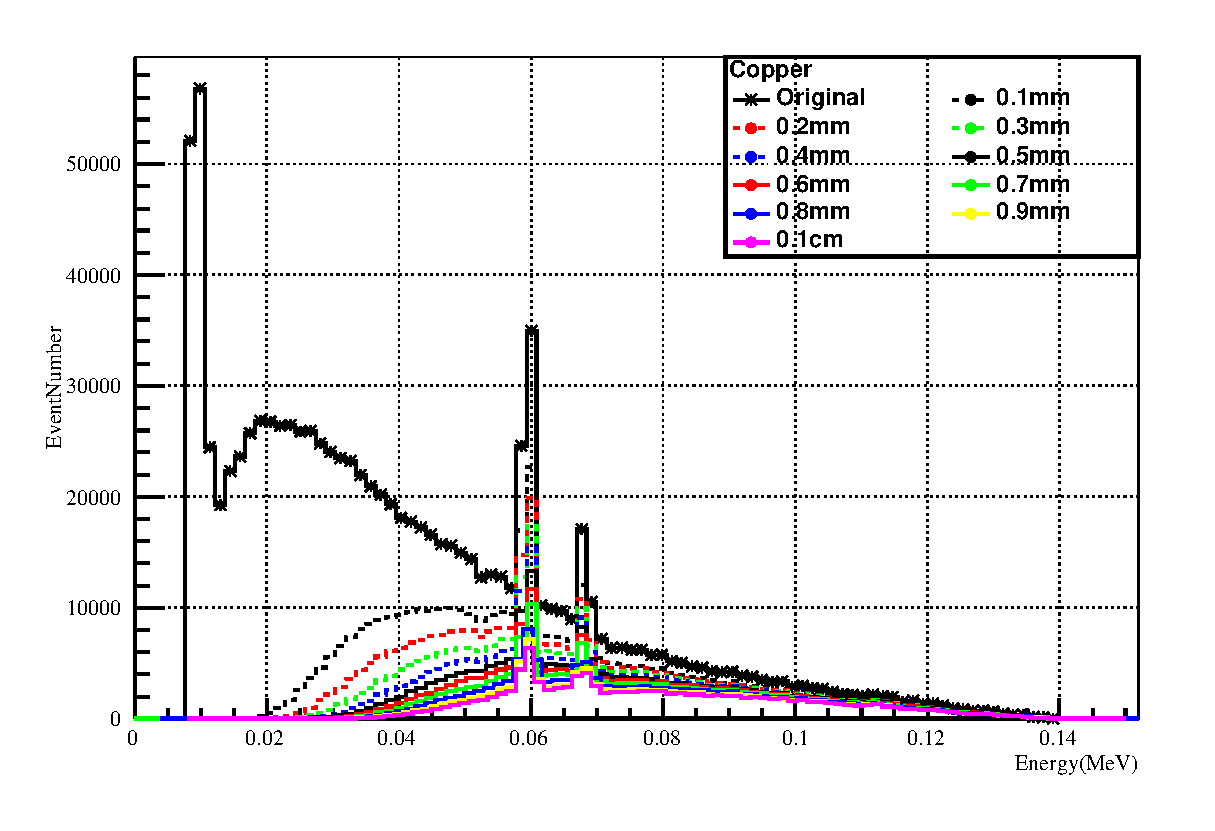
\includegraphics[width=\textwidth,height=0.58\textwidth]{140keVelectronEnergyAfterCopperApron.eps}
      \end{figure}
    \end{minipage}
  \end{frame}
  %--------------------------------
  \begin{frame}\frametitle{不同能量阈值下光子数的比例}
    \begin{figure}[ht]
      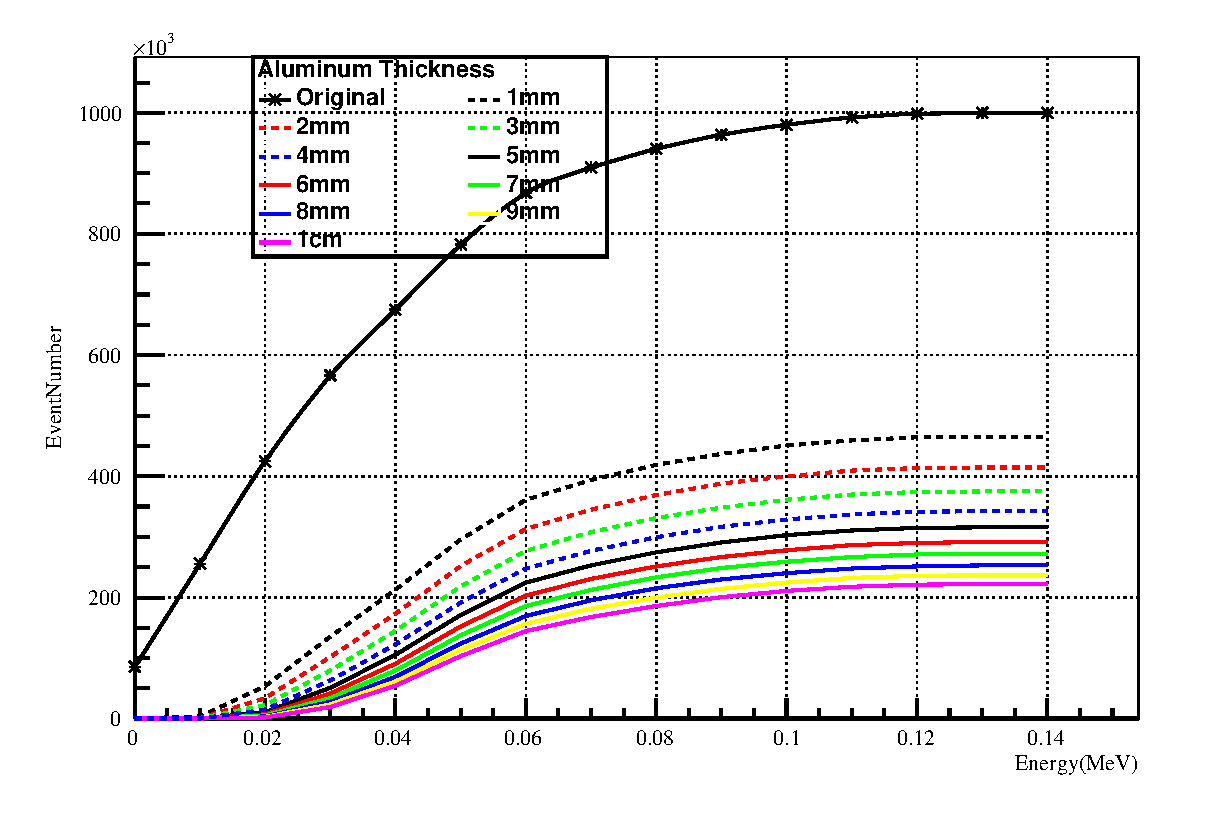
\includegraphics[width=0.5\textwidth]{140keVElectronXrayAluminumDistribution.eps}~
      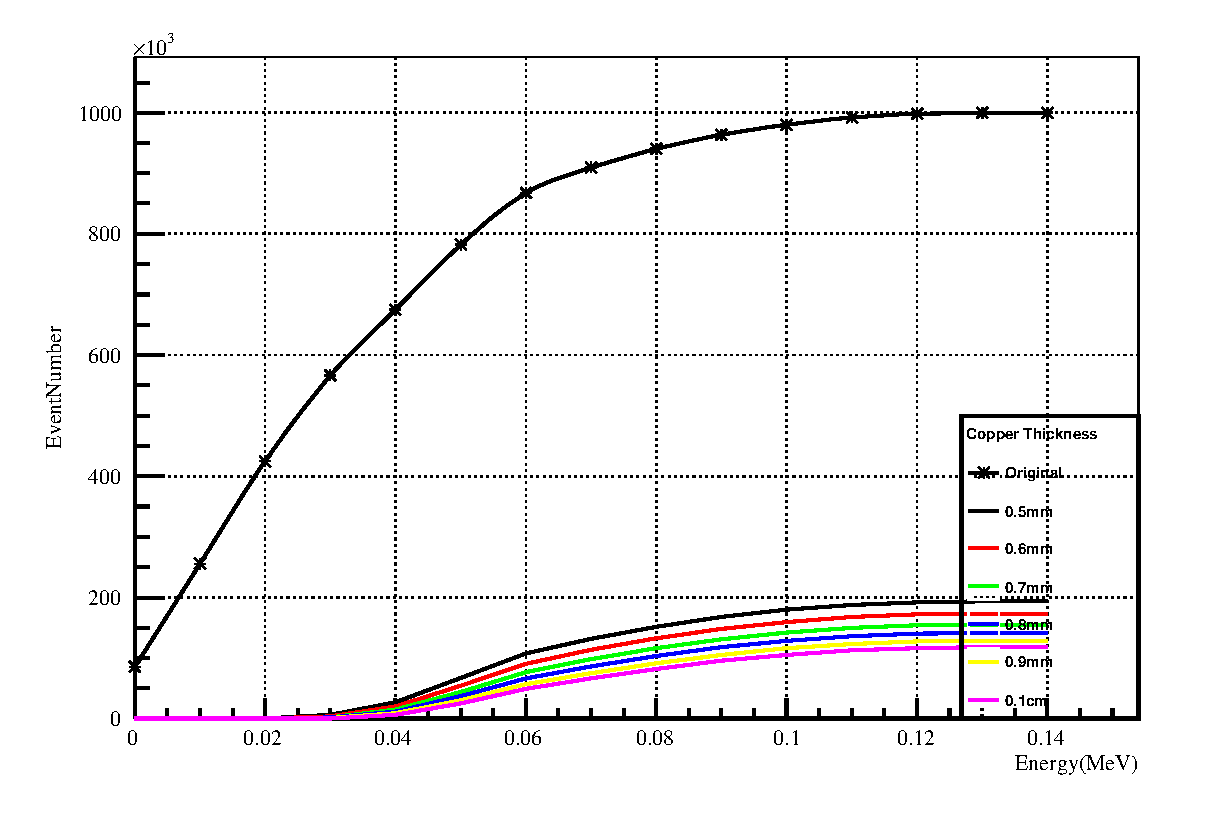
\includegraphics[width=0.5\textwidth]{140keVElectronXrayCopperDistribution.eps}

      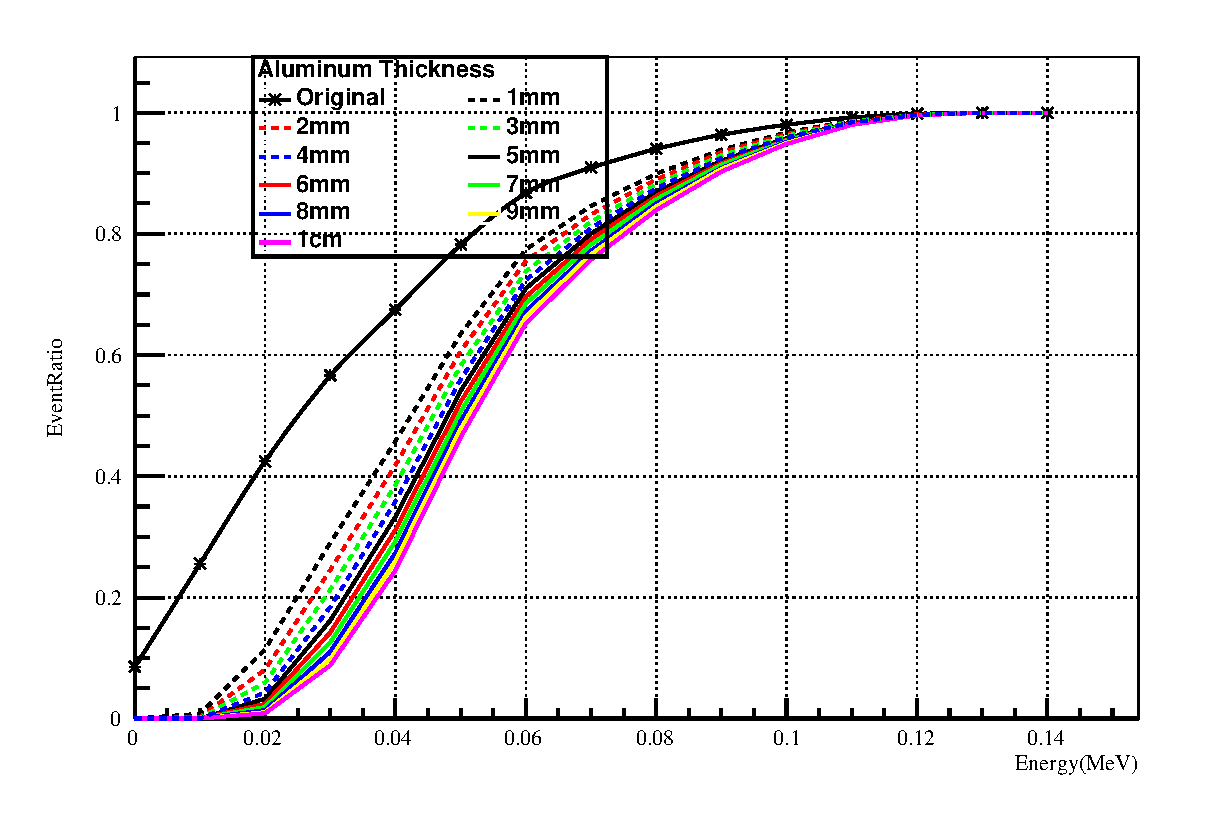
\includegraphics[width=0.5\textwidth]{140keVElectronXrayAluminumDistributionRatio.eps}~
      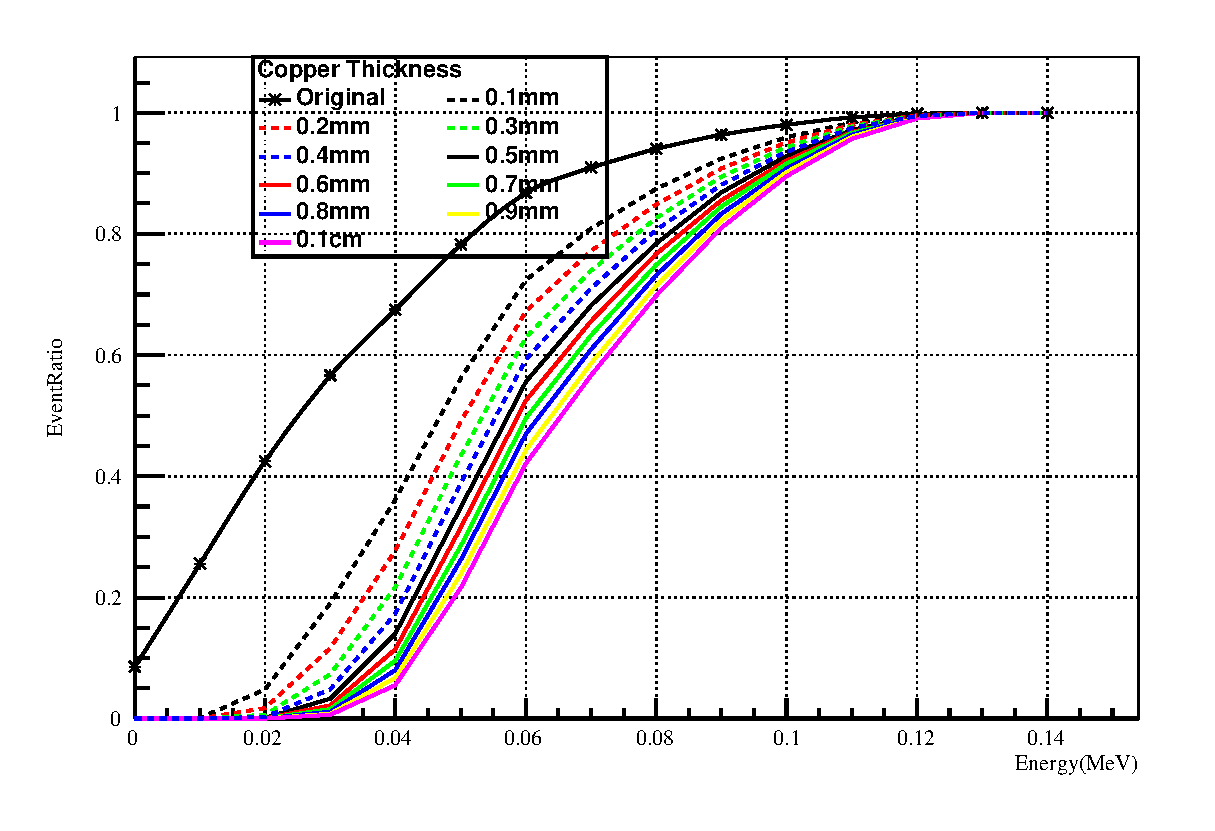
\includegraphics[width=0.5\textwidth]{140keVElectronXrayCopperDistributionRatio.eps}
    \end{figure}
  \end{frame}
  %--------------------------------------
  \section{重建算法及FDK代码}
  \begin{frame}\frametitle{ROOT准备}
    \begin{minipage}[t]{0.5\textwidth}
      \vskip 0.5cm
      \liuhao
      CT图像为灰度图像,平时都没用过灰度图像,所以首先学习了如何用ROOT画出灰度图片。
      学习之后发现其实也很简单,只需要设置灰度条的颜色数目及变化方式即可,还可以使图像
      更细腻。
      \vskip 0.5cm
      \begin{figure}[ht]
	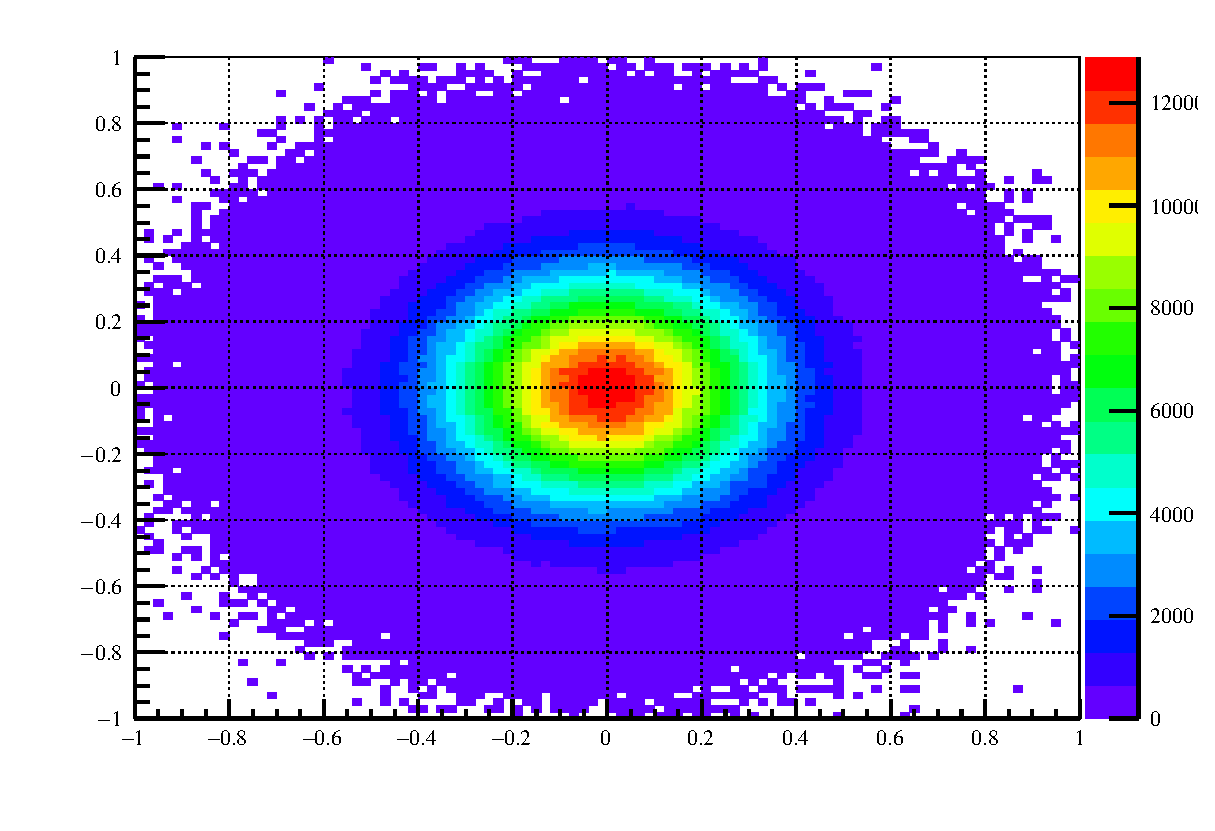
\includegraphics[width=\textwidth]{Test.eps}
      \end{figure}
    \end{minipage}
    \pause
    \begin{minipage}[t]{0.5\textwidth}
      \begin{figure}[ht]
	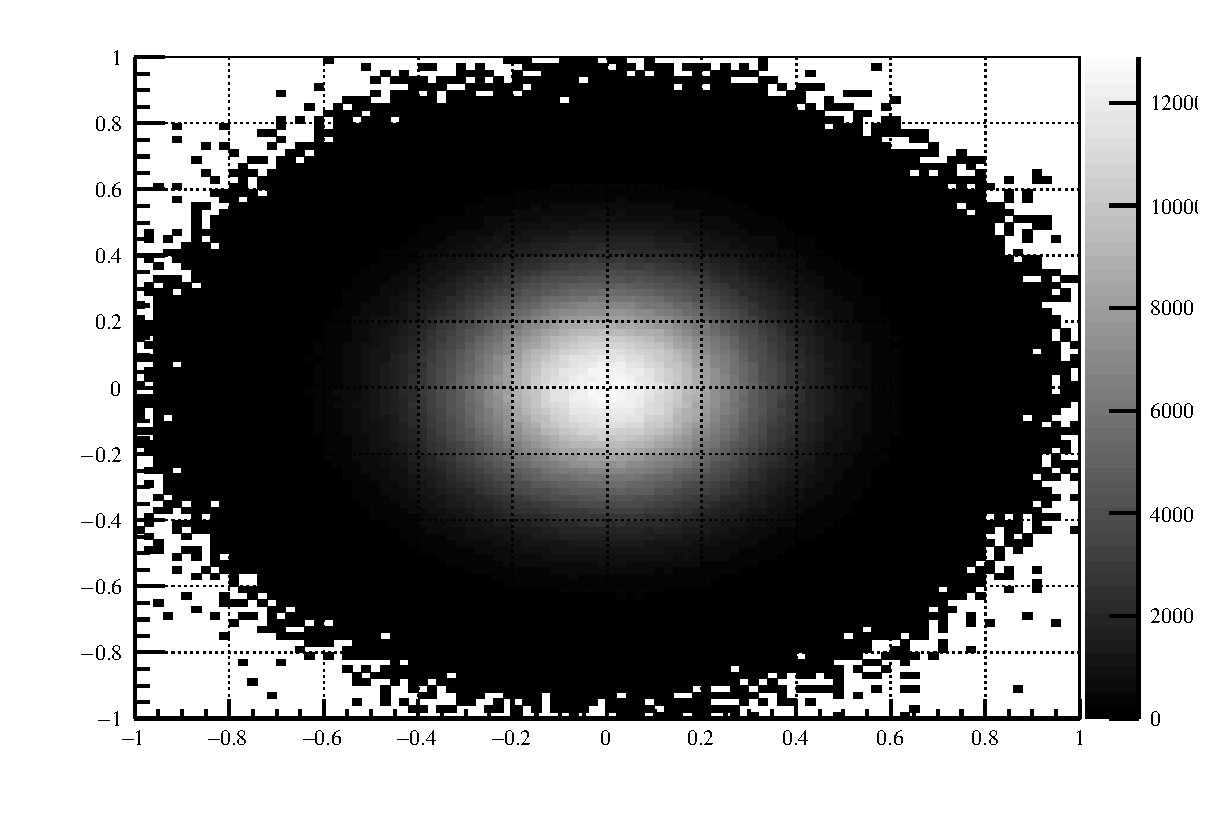
\includegraphics[width=\textwidth]{TestGrayStyle.eps}

	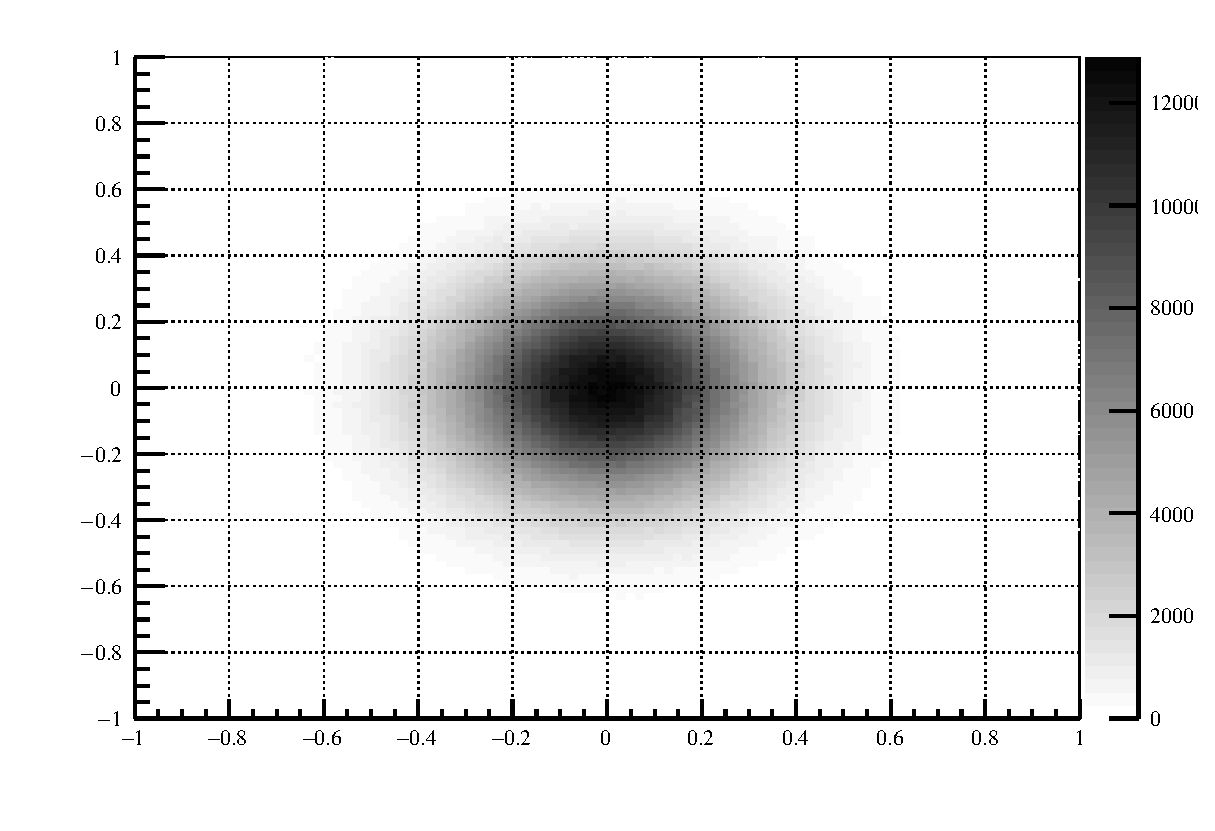
\includegraphics[width=\textwidth]{TestGrayStyleBack.eps}
      \end{figure}
    \end{minipage}
  \end{frame}
  %-----------------------------
  \begin{frame}\frametitle{编写Makefile}
    \begin{minipage}[t]{0.3\textwidth}
      \liuhao
      Linux下编译代码一般自己编写Makefile(类似于
      
      windows下的projects)或
      者CMakeLists。以前写的GNUmakefile稍微修改就可以直接使用,但仅限于Linux平台,cmake
      是一种跨平台的编译方式,可以用简单的语句来描述所有平台的编译过程。FDKSim代码却重建出
      一幅点阵图。
      \begin{itemize}
	\item 阅读FDKSim代
	  
	  码。
      \end{itemize}
    \end{minipage}
    \begin{minipage}[t]{0.7\textwidth}
      \begin{figure}[ht]
        \includegraphics[width=\textwidth]{Recons.eps}
	\caption{\liuhao data.txt重建结果} 
      \end{figure}
    \end{minipage}
  \end{frame}
%=========================================
  \ThankYouPage
\end{CJK*}
\end{document}
